% Szglab4
% ===========================================================================
%

\newcommand{\define}[2]{\textbf{#1}\hspace{3mm}#2\medskip\newline}

\chapter{Követelmény, projekt, funkcionalitás}

\thispagestyle{fancy}

\section{Bevezetés}

\subsection{Cél}
A projekt követelményeinek, alapvető felépítésének és funkcionalitásának ismertetése; ezek segítségével körbehatárolni a fejlesztés menetét és a végleges program felépítését, működését. Fejlesztés közben ezeket folyamatosan figyelembe kell majd venni, eltérni tőlük nem szabad.

\subsection{Szakterület}
Az elkészítendő szoftver egy számítógépes játék, így nem egy kifejezett szakterület részére készül, hanem általános felhasználásra, szórakoztatásra. A játék az úgynevezett ``tower defense'' kategóriába sorolható, ezért azoknak ajánlott, akik szeretik az ilyen típusú játékokat.

\subsection{Definíciók, rövidítések}
\define{architekturális kép}{A szoftver belső felépítését szemléltető ábra.}
\define{archívum}{Olyan számítógépes fájl, amely több másik fájlt foglal magában.}
\define{BME}{Budapest Műszaki Egyetem rövidítése.}
\define{Eclipse}{Fejlesztőkörnyezet főként a Java programozási nyelvhez.}
\define{Enterprise Architect}{Egy UML diagramok készítését lehetővé tevő szoftver.}
\define{Facebook}{Internetes közösségi oldal}
\define{fejlesztőkörnyezet}{Olyan számítógépes program vagy programok összessége, ami lehetővé teszi vagy leegyszerűsíti egy fejlesztési munka végrehajtását.}
\define{funkció}{A program működésének egy külön megfogalmazható része.}
\define{Git}{Egy verziókezelő rendszer.}
\define{GitHub}{A Git verziókezelő rendszerre épülő internetes szolgáltatás.}
\define{HSZK}{Hallgatói Számítógép Központ rövidítése.}
\define{háttértár}{A számítógépnek egy olyan tárhelye, ami a számítógép kikapcsolása után is megőrzi az adatokat.}
\define{IntelliJ IDEA}{Fejlesztőkörnyezet főként a Java programozási nyelvhez.}
\define{jar}{A Java programozási nyelv által használt fájltípus; egy archívum, amiben egy adott program vagy programmodul futtatásához szükséges fájlok vannak.}
\define{JRE6}{Java Runtime Environment 6 rövidítése. Ez egy olyan program, ami szükséges a Java programozási nyelvben írt programok használatához.}
\define{PC}{Personal Computer rövidítése, jelentése személyi számítógép.}
\define{proto/prototípus}{A program olyan állapota, amikor minden belső működés meg van valósítva és működik, de grafikus felület még nincsen hozzá.}
\define{Skype}{Egy interneten keresztüli telefonálásra használható program.}
\define{szkeleton}{A program olyan állapota, amikor a program belső felépítése készen van, de nem csinál semmit.}
\define{szoftver}{Számítógépen futtatható program.}
\define{TeX}{Dokumentum formázó és betűszedő rendszer, segítségével magas színvonalú szöveges dokumentumok hozhatók létre (pl. ez a dokumentáciő).}
\define{TeXworks}{Fejlesztőkörnyezet TeX-hez.}
\define{UML}{Unified Modeling Language rövidítése, egy rendszer modelező eszköz.}
\define{use-case}{Egy felhasználó és egy rendszer közötti, adott célt elérő interakció leírása.}
\define{verziókezelő}{Olyan számítógépes program, aminek segítségével eltárolható fájloknak régebbi verziói, így később vissza lehet térni egy adott verzióhoz, illetve nyomon lehet követni egy fájl változását.}
\define{wiki}{Egy olyan weboldal, aminek tartalmát a felhasználók szerkeszthetik, így mindenki hozzáadhatja a saját tudását egy adott témához.}

\subsection{Hivatkozások}
Szoftver labor 4 - \url{https://www.iit.bme.hu/~szoftlab4/}

\subsection{Összefoglalás}
A dokumentum további részeiben található:
\begin{itemize}
\item Áttekintés, ami nagyvonalakban bemutatja a szoftvert
\item A szoftverrel kapcsolatos követelmények leírása, később ezek figyelembevételével kell a programot fejleszteni
\item Lényegesebb use-case-ek felsorolása
\item Szótár, ami a szoftverrel kapcsolatos nem hétköznapi, illetve nem hétköznapi értelmében használt szavak definícióit tartalmazza
\item A projekt kivitelezésének terve
\item Projekt napló
\end{itemize}

\begin{nopb}
\section{Áttekintés}
\subsection{Általános áttekintés}
% \comment{A kialakítandó szoftver legmagasabb szintű architekturális képe. A fontosabb alrendszerek felsorolása, a közöttük kialakítandó interfészek lényege, a felhasználói kapcsolatok alapja. Esetleges hálózati és adattárolási elvárások.}


A szoftver legmagasabb szintű architekturális képe:
\newline
\begin{figure}[H]
\centering
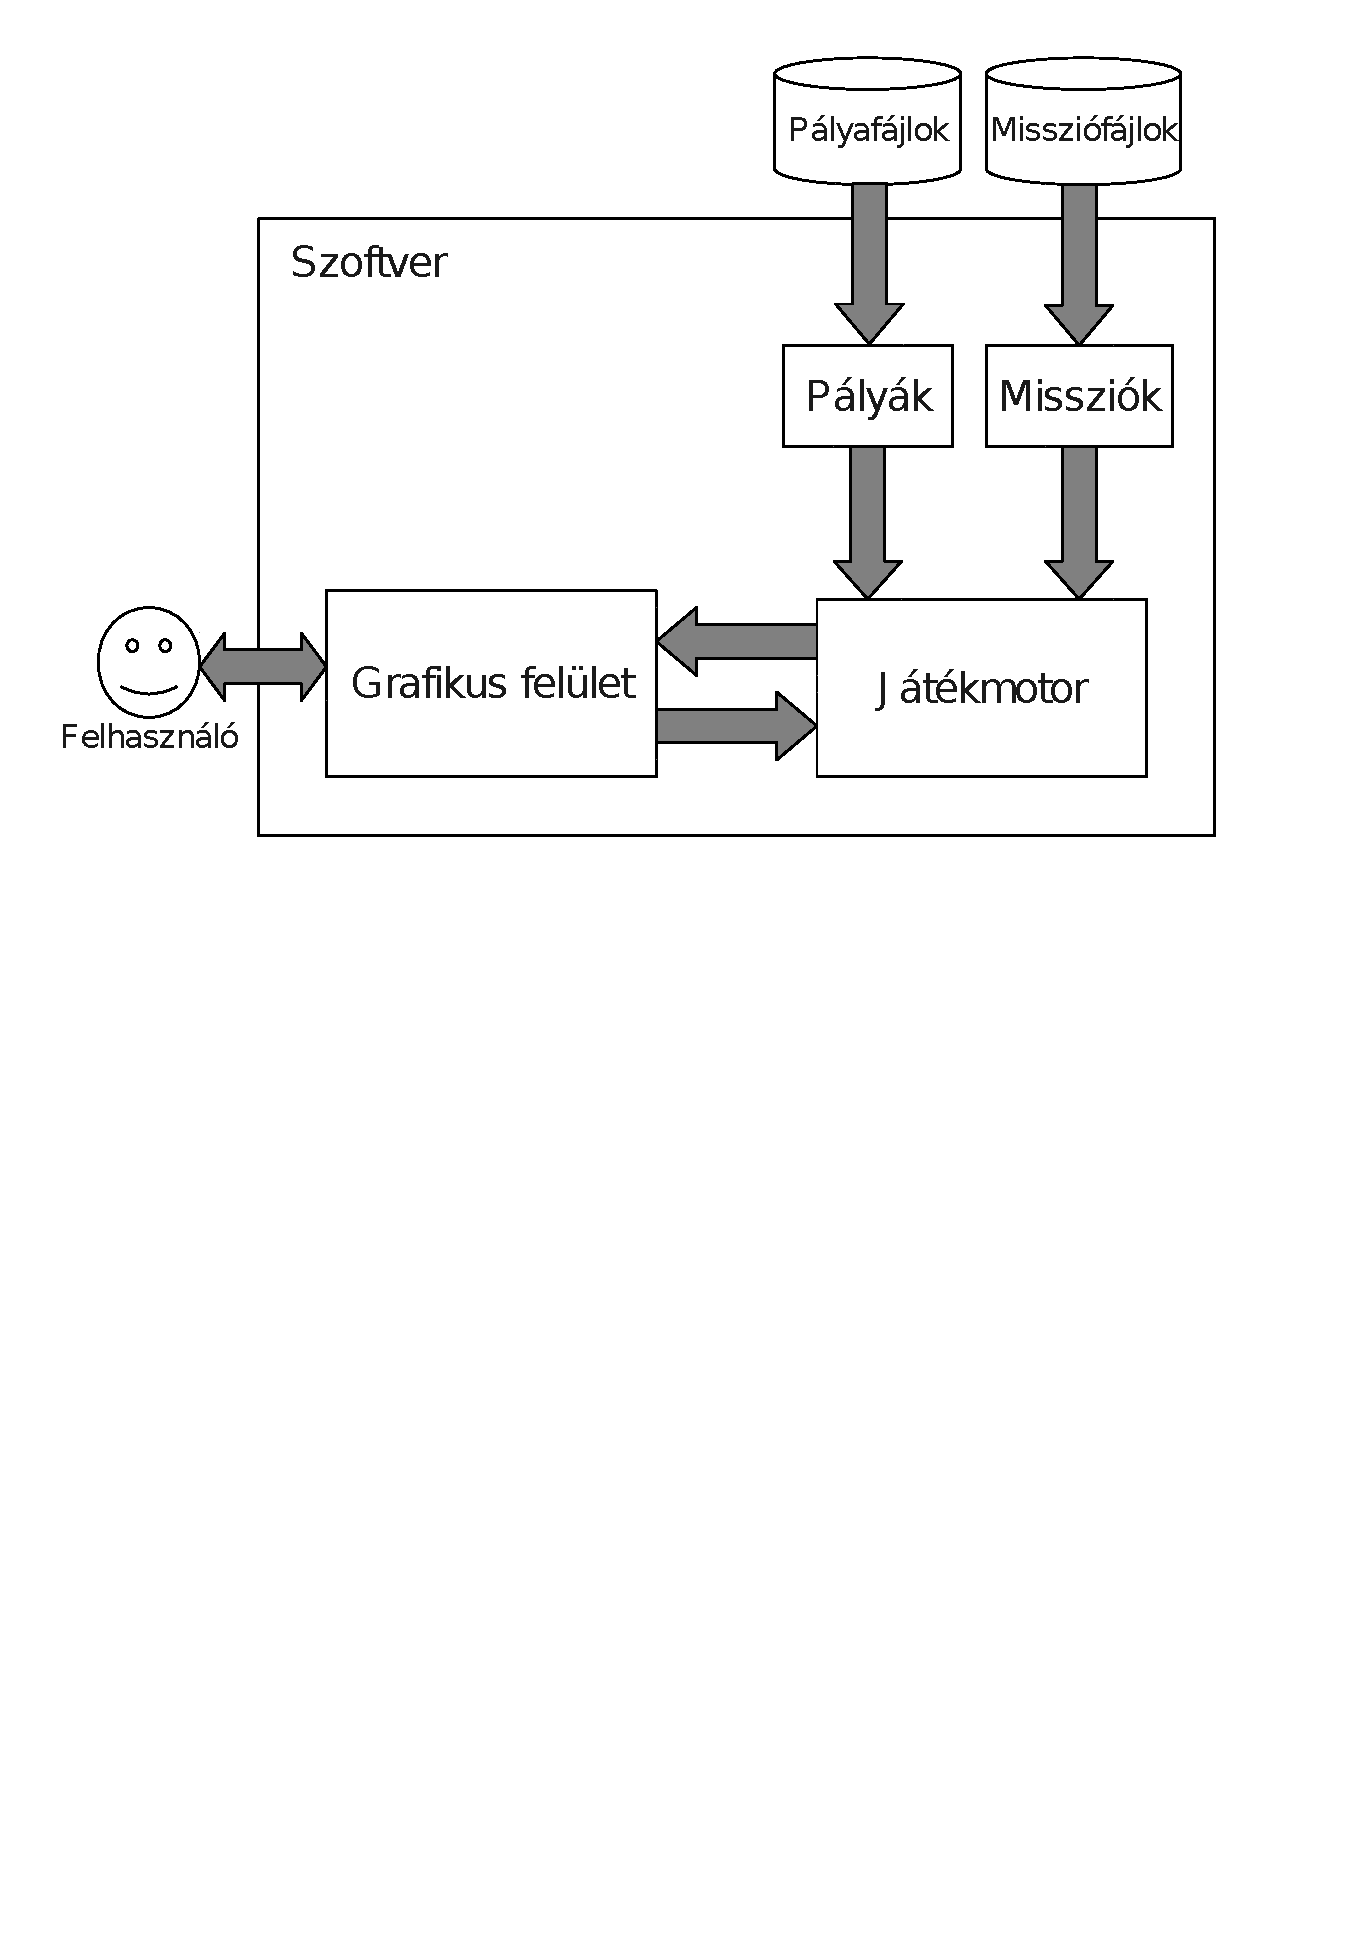
\includegraphics[scale=.7]{images/arch.eps}
\caption{Architekturális kep}
\label{overflow}
\end{figure}
\end{nopb}
A szoftver legfontosabb alrendszere a Játékmotor. Ebben zajlik a tulajdonképpeni játék, ez futtatja a logikát, ami által az egységek belépnek, és haladnak végig az utakon a Végzet Hegye felé, ez tartja számon a tornyokat, azok fejlesztéseit, ez gondoskodik arról, hogy minden torony a megfelelő egységet sebezze, a megfelelő módon és mértékben. A pályát (az utak elrendezését) a Pályák alrendszertől kéri le, és a forgatókönyvet, ami szerint belépnek az egységek, pedig a Missziók alrendszertől. A pillanatnyi állapotot, amely a kirajzoláshoz szükséges, szolgáltatja a Grafikus felület felé, valamint végrehajtandó parancsokat, vezérlést fogad attól. \\ \\
A Pályák alrendszer egyszerűen betölti a Pályafájlokból a pályákat, nyilván tartja, és a Játékmotor rendelkezésére bocsátja őket. \\ \\
A Missziók alrendszer a Pályák-hoz nagyon hasonlóan a Missziófájlokból betölti a missziókat, nyilván tartja, és a Játékmotor rendelkezésére bocsátja őket. \\ \\
A Grafikus felület egyrészt a játék megjelenítését szolgálja a Felhasználó felé, másrészt ezen keresztül irányítható a Játékmotor. \\ \\
Hálózatot a szoftver egyáltalán nem használ. Háttértáron pedig a program saját fájljai - .jar archivum(ok), a kirajzoláshoz szükséges képek, és az egyes pályákat, valamint missziókat tároló fájlok - számára kell helyet biztosítani. Ezeken kívül nincs további futási idejű tárhelyigénye.

\subsection{Funkciók}
% \comment{A feladat kb. 4000 karakteres (kb 1,5 oldal) részletezettségű magyar nyelvű leírása. Nem szerepelhetnek informatikai kifejezések.}

A szoftver egy úgynevezett tower defense játék. Az ilyen játékok lényege általában az, hogy a pályán lévő, kijelölt úton különböző ellenséges egységek indulnak el a belépési pontból a céljuk felé. A játékos feladata pedig az, hogy ezt megakadályozza azzal, hogy az út mentén valamilyen erőforrásokat felhasználva tornyokat épít, amelyek a hozzájuk elég közel kerülő egységeket bizonyos mértékben és időközönként sebzik, ezzel életerejüket folyamatosan csökkentik. Ha egy egység életereje elfogy, megáll, elpusztul, eltűnik, és további fenyegetést nem jelent. \\ \\
A játék akkor ér véget, ha minden ellenséget elpusztítottunk, ezzel megvédtük a célt, vagy ha legalább egy ellenség célba ér. Előbbi esetben a játékos nyer, utóbbi esetben a játékos veszít, az ellenség pedig fényes győzelmet arat és örökké uralja a világot. \\ \\
Ebben a konkrét esetben a játéktér a Középföldén elfekvő Mordorban található, az ellenségek az ádáz Gyűrű Szövetségének tagjai, akik lehetnek emberek, tündék, törpök vagy hobbitok, és céljuk a Végzet Hegye, amelyben az Egy Gyűrűt szándékoznak elpusztítani. Minden ellenségtípus eltérő tulajdonságokkal (sebesség, életerő, stb.) rendelkezik. Például egy törp lassabb, mint egy tünde, de több az életereje. Egy ember pedig gyorsabb egy törpnél, de szívósabb, mint egy tünde. A hobbitok pedig általában népes csoportokban érkeznek, így lassúságuk és kevés életerejük ellenére komoly kihívást jelenthetnek. \\ \\
A játékos, aki a jóságos Szarumánt személyesíti meg, ezt nem hagyhatja, hiszen így felettese, Szauron is odaveszne. A védekező tornyok felépítéséhez varázserejét tudja felhasználni, amely minden ellenséges egység elpusztításakor bizonyos mértékben megnő. \\ \\
Ezen kívül lehetősége van - szintén varázserejét elköltve - a tornyait különböző mágikus kövekkel ellátni, így azok bizonyos típusú ellenség esetén nagyobbat sebeznek. Más kövek növelik a tornyok tüzelési gyakoriságát vagy hatótávolságát. \\ \\
Az utakra építhet akadályokat, amelyekre érve az egységek lelassulnak, így esetleg tovább tartózkodnak a tornyok hatókörében, azoknak több esélyük van megsebezni őket. \\ \\
A tornyokon kívül a játékosnak lehetősége van akadályokat is felruházni varázskövekkel. A varázskövekkel felruházott akadályok jobban lelassítják a beléjük érkező ellenségeket. A lassítás mértéke függ az ellenség típusától. \\ \\
Egyes pályákon több belépési pont és több, a célba vezető kijárat is szerepelhet, és azokat összetett úthálózat is összekötheti, amelyen az egységek véletlenszerű útvonalakat választanak ki.
A támadás több hullámban történik, minden hullámban egy bizonyos időben minden típusú ellenségből meghatározott létszámú csoport jön, adott késleltetéssel egymáshoz képest. A hullámok leírását minden pályához missziók tartalmazzák, amelyek így lehetnek eltérő nehézségűek vagy hangulatúak. \\ \\

\subsection{Felhasználók}
% \comment{A felhasználók jellemzői, tulajdonságai}
A szoftver felhasználói számára nincs szükség különösebb előképzettségre, a használata rövid időn belül elsajátítható, és a játék élvezhető bárki számára, aki a szótárban felsorolt definiciókat képes értelmezni.

\subsection{Korlátozások}
% \comment{Az elkészítendő szoftverre vonatkozó – általában nem funkcionális - előírások, korlátozások.}
A szoftverre vonatkozó előírás és korlátozás is egyben egyedül az, hogy a standard Java könyvtárkészletet kell használnia, és semmilyen más csomagot nem vehet igénybe.

\subsection{Feltételezések, kapcsolatok}
% \comment{A dokumentumban használt anyagok, web-oldalak felsorolása}
Szoftver labor 4 feladatkiírás - \url{https://www.iit.bme.hu/~szoftlab4/feladat.shtml}

\section{Követelmények}
\subsection{Funkcionális követelmények}

% \comment{Az alábbi táblázat kitöltésével készítendő. Dolgozzon ki követelmény azonosító rendszert! Az ellenőrzés módja szokásosan bemutatás és/vagy kiértékelés. Prioritás lehet alapvető, fontos, opcionális. Az alapvető követelmények nem teljesítése végzetes. Forrás alatt a követelményt előíró anyagot, szervezetet kell érteni. Esetünkben forrás lehet maga a csapat is, mikor ő talál ki követelményt. Use-case-ek alatt az adott követelményt megvalósító használati esete(ke)t kell megadni.}

% Azonosító, Leírás, Ellenőrzés, Prioritás, Forrás, Use-case, Komment
\begin{longtable}{| p{16mm} | p{4cm} | l | l | l | p{15mm} | p{2cm} |}
\hline
\textbf{Azonosító}   & \textbf{Leírás} & \textbf{Ellenőrzés} & \textbf{Prioritás} & \textbf{Forrás} & \textbf{Use-case} & \textbf{Komment} \tabularnewline
\hline\hline
1.01 & Tornyokat lehet építeni & bemutatás & alapvető & megrendelő & Torony építése &  \tabularnewline
\hline
1.02 & Az ellenségek igyekszenek eljutni a célig & bemutatás & alapvető & megrendelő &  & \tabularnewline
\hline
1.03 & A tornyok képesek lőni & bemutatás & alapvető & megrendelő &  &  \tabularnewline
\hline
1.04 & Az ellenségek sebződnek a tornyok lövedékétől & kiértékelés & alapvető & megrendelő &  &  \tabularnewline
\hline
1.05 & Az ellenségek bizonyos mértékű sebződés után meghalnak & bemutatás & alapvető & megrendelő &  & \tabularnewline
\hline
1.06 & Az elpusztított ellenségek után varázserőt kap a játékos & bemutatás & alapvető & megrendelő &  &  \tabularnewline
\hline
1.07 & A különböző ellenségek, különböző tulajdonságokkal rendelkezeknek & bemutatás & opcionális & csapat &  & Különböző életerő, sebesség \tabularnewline
\hline
1.08 & Vannak utak & bemutatás & alapvető & megrendelő &  &  \tabularnewline
\hline
1.09 & Az ellenségek az utakról nem térnek le & bemutatás & alapvető & megrendelő &  &  \tabularnewline
\hline
1.10 & Tornyot nem lehet útra építeni & bemutatás & fontos & megrendelő & Torony építése &  \tabularnewline
\hline
1.11 & Akadályokat lehet építeni & bemutatás & alapvető & megrendelő & Akadály építése &  \tabularnewline
\hline
1.12 & Akadályt csak útra lehet rakni & bemutatás & fontos & megrendelő & Akadály építése &  \tabularnewline
\hline
1.13 & Az akadályok lassítják az ellenségeket & bemutatás & fontos & megrendelő &  &  \tabularnewline
\hline
1.14 & A tornyoknak van tüzelési gyakorisága, hatótávolsága & bemutatás & alapvető & megrendelő &  &  \tabularnewline
\hline
1.15 & Tornyokat és akadályokat varázskövekkel lehet ellátni & bemutatás & alapvető & megrendelő & Torony/ akadály echant-olás &  \tabularnewline
\hline
1.16 & Különböző varázskövek vannak & bemutatás & opcionális & megrendelő &  &  \tabularnewline
\hline
1.17 & Idővel egyre gyakrabban érkeznek ellenségek, egyre nagyobb csoportban & bemutatás & fontos & megrendelő &  &  \tabularnewline
\hline
1.18 & A játékot el lehet indítani & bemutatás & alapvető & megrendelő & Új játék indítása &  \tabularnewline
\hline
1.19 & A játékot fel lehet adni & bemutatás & opcionális & csapat & Feladás &  \tabularnewline
\hline
1.20 & Több pálya van & bemutatás & opcionális & csapat & Pálya kiválasztása &  \tabularnewline
\hline
1.21 & A játékból ki lehet lépni & bemutatás & alapvető & csapat & Kilépés &  \tabularnewline
\hline
1.22 & Ha az összes ellenség meghalt, a játékos nyer & bemutatás & alapvető & csapat &  &  \tabularnewline
\hline
1.23 & Több útvonal vezet a célig & bemutatás & alapvető & csapat &  &  \tabularnewline
\hline
1.24 & Ha egy ellenség eljut a célig, a játékos veszít & bemutatás & alapvető & csapat &  &  \tabularnewline
\hline
\end{longtable}

\subsection{Erőforrásokkal kapcsolatos követelmények}

% \comment{A szoftver fejlesztésével és használatával kapcsolatos számítógépes, hardveres, alapszoftveres és egyéb architekturális és logisztikai követelmények}

% Azonosító, Leírás, Ellenőrzés, Prioritás, Forrás, Komment
\begin{longtable}{| l | p{5cm} | l | l | l | l |}
\hline
\textbf{Azonosító}   & \textbf{Leírás} & \textbf{Ellenőrzés} & \textbf{Prioritás} & \textbf{Forrás} & \textbf{Komment} \tabularnewline
\hline\hline
2.01 & Git & nincs  & alapvető & csapat & Elosztott verziókezelő \tabularnewline
\hline
2.02 & Github account & nincs  & alapvető & csapat & Git tárhely \tabularnewline
\hline
2.03 & JRE6 & bemutatás  & alapvető & megrendelő & \tabularnewline
\hline
2.04 & Eclipse & nincs & opcionális & csapat & Java IDE \tabularnewline
\hline
2.05 & IntelliJ IDEA & nincs & opcionális & csapat & Java IDE \tabularnewline
\hline
2.06 & HSZK-ban találhatókkal azonos vagy jobb teljesítményű PC & bemutatás & alapvető & megrendelő &  \tabularnewline
\hline
2.07 & Monitor & nincs & alapvető & csapat &  \tabularnewline
\hline
2.08 & Egér & nincs & alapvető & csapat &  \tabularnewline
\hline
2.09 & Enterprise Architect & nincs & opcionális & csapat & UML modellező \tabularnewline
\hline
2.10 & TeXworks & nincs & opcionális & csapat & LaTeX editor \tabularnewline
\hline
\end{longtable}


\subsection{Átadással kapcsolatos követelmények}
% \comment{A szoftver átadásával, telepítésével, üzembe helyezésével kapcsolatos követelmények}

% Azonosító, Leírás, Ellenőrzés, Prioritás, Forrás, Komment
\begin{longtable}{| l | p{5cm} | l | l | l | l |}
\hline
\textbf{Azonosító}   & \textbf{Leírás} & \textbf{Ellenőrzés} & \textbf{Prioritás} & \textbf{Forrás} & \textbf{Komment} \tabularnewline
\hline\hline
3.01 & Szkeleton átadás & bemutatás & alapvető & megrendelő & márc. 26. \tabularnewline
\hline
3.02 & Proto átadás & bemutatás & alapvető & megrendelő & ápr. 23. \tabularnewline
\hline
3.03 & Teljes program átadása & bemutatás & alapvető & megrendelő & máj. 14. \tabularnewline
\hline
3.04 & Útmutató alapján telepíthető, külső segítség nélkül & bemutatás & fontos & megrendelő &  \tabularnewline
\hline
3.05 & A programnak működnie kell a BME HSZK számítógépein & bemutatás & alapvető & megrendelő &  \tabularnewline
\hline
\end{longtable}

\subsection{Egyéb nem funkcionális követelmények}
% \comment{A biztonsággal, hordozhatósággal, megbízhatósággal, tesztelhetőséggel, a felhasználóval kapcsolatos követelmények}

Nincs egyéb nem funkcionális követelmény.

% Azonosító, Leírás, Ellenőrzés, Prioritás, Forrás, Komment
% \begin{longtable}{| l | l | l | l | l | l |}
% \hline
% \textbf{Azonosító}   & \textbf{Leírás} & \textbf{Ellenőrzés} & \textbf{Prioritás} & \textbf{Forrás} & \textbf{Komment} \tabularnewline
% \hline\hline
% 4.01 & ... &  & alapvető & megrendelő & ... \tabularnewline
% \hline
% \end{longtable}


\section{Lényeges use-case-ek}
% \comment{A 2.3.1-ben felsorolt követelmények közül az alapvető és fontos követelményekhez tartozó használati esetek megadása az alábbi táblázatos formában.}

\subsection{Use-case leírások}

\usecase
{Új játék indítása}
{Új játék indul el}
{Játékos}
{1. A játékos kiválasztja a menüben az ``Új játék'' feliratú gombot, és megnyomja. \newline
2. Ezután kiválaszthatja  a nehézséget és a pályát. \newline
3. Elindul a játék a kiválasztott pályával és nehézséggel.}

\usecase
{Pálya kiválasztása}
{Ki kell választani a pályát amelyen játszani kíván.}
{Játékos}
{Új játék indítása után egy listából ki kell választani a pályát amelyen játszani kíván.}

\usecase
{Nehézségi szint kiválasztása}
{Ki kell választani, hogy milyen nehézségen kíván játszani.}
{Játékos}
{Új játék indítása, és a pálya kiválasztása után, ki kell választani három opció közül,
 hogy mennyire legyen a játék nehéz.}

\usecase
{Torony építése}
{Új tornyot épít}
{Játékos}
{Olyan mezőre kattintva, ahol nincsen út vagy torony, ott új torony épül,
ha van elég varázserő hozzá.}

\usecase
{Akadály építése}
{Új akadályt épít}
{Játékos}
{Olyan mezőre kattintva ahol út van, és még nincsen akadály, ott akadály épül,
ha van elég varázserő hozzá.}

\usecase
{Torony/akadály enchant-olás}
{Már létező tornyot vagy akadályt enchant-olunk}
{Játékos}
{Toronyra vagy akadályra kattintva ki kell választani, hogy milyen drágakővel szeretné enchant-olni,
és ha van elég varázserő hozzá akkor megtörténik az enchant.}

\pagebreak

\usecase
{Feladás}
{Feladjuk a jelenlegi játékot}
{Játékos}
{A feladás gombra kattintva a játék végetér, és megnyílik a főmenü.}

\usecase
{Kilépés}
{Kilép az alkalmazásból}
{Játékos}
{Az ablak jobb felső sarkában, a bezárásra kattintva az alkalmazás kilép.}

\subsection{Use-case diagram}

\begin{figure}[ht!]
\centering
\includegraphics[width=170mm]{images/UseCase.png}
\caption{Use-case diagram}
\label{overflow}
\end{figure}

\section{Szótár}
% \comment{A szótár a követelmények alapján készítendő fejezet. Egy szótári bejegyzés definiálásához csak más szótári bejegyzések és köznapi – a feladattól független – fogalmak használhatók fel. A szótár mérete kb. 1-2 oldal legyen.}\newline

\define{akadály}{A játékos készítheti, az utakra lehet építeni. A rajta áthaladó ellenségeket lelassítja. Lehet enchantolni.}
\define{cél}{A pályán kijelölt hely; ha ide eljutnak az ellenségek, akkor vége a játéknak és a játékos vesztett.}
\define{életerő}{Egy szám, ami minden ellenséghez rendelve van. Ha ez a szám eléri a 0-t vagy kisebb lesz, az ellenség meghal.}
\define{ellenség}{A pályán az utakon haladnak, van egy életerő tulajdonságuk, ami lövés hatására csökken, majd ha eléri a 0-t, akkor az ellenség meghal.}
\define{enchantolás}{Torony vagy akadály varázskővel való felruházása.}
\define{építés}{A játékos által egy torony vagy akadály elhelyezése a játéktérre.}
\define{hatótávolság}{A tornyok tulajdonsága, azt határozza meg, hogy a torony milyen messzire tud lőni.}
\define{játék elvesztése}{A játék egy lehetséges végződése, akkor következik be, ha egy ellenség elér a célhoz.}
\define{játék megnyerése}{A játék egy lehetséges végződése, akkor következik be, az összes ellenség meghal anélkül, hogy elérnének a célhoz.}
\define{lövés}{Az az esemény, amikor a torony egy a hatótávolságán belül lévő ellenség életerejét csökkenti.}
\define{meghal}{Az az esemény, amikor egy ellenség életereje eléri a 0-t.}
\define{nehézség}{A játék különböző tulajdonságainak egy adott beállítása, ezzel változtatható, hogy milyen nehéz teljesíteni a játékot.}
\define{út}{A pályán kijelölt rész, amin az ellenségek eljuthatnak a célig. Az ellenségek csak ezen haladhatnak, az akadályokat csak erre szabad építeni, a tornyokat viszont az utakra nem lehet építeni.}
\define{pálya}{Az a tér, amin a játék zajlik; ezen vannak az utak, és erre lehet építeni a tornyokat és akadályokat.}
\define{sebződés}{Ha egy ellenség sebződést kap, akkor lemegy az életereje.}
\define{torony}{A játékos által készíthető dolgok közül a fontosabb; ezzel lehet megakadályozni az ellenségek célhoz jutását. Lőni tud, és lehet enchantolni.}
\define{tower defense}{Egy játékműfaj, amelyben a játék célja, hogy a pályán áthaladni próbáló ellenségeket megakadályozzuk abban, hogy elérjék a célt. Ezt tornyok és akadályok segítségével érhetjük el.}
\define{tüzelési gyakoriság}{A tornyok tulajdonsága, azt határozza meg, hogy egy adott idő alatt mennyi lövést tud leadni egy torony.}
\define{varázserő}{A játékos tulajdonsága; egy mennyiség, az ellenségek elpusztulásakor növekszik, torony és akadály építésekor és enchantoláskor pedig csökken. A játékos csak akkor tud építeni és enchantolni, ha a jelenlegi varázserő több, mint amennyi az építéshez vagy enchantoláshoz szükséges.}
\define{varázskő}{Olyan játékelem, amit hozzá lehet rendelni tornyokhoz és akadályokhoz (enchantolás), ami ettől valamilyen szempontból jobb lesz, pl. tüzelési gyakoriság növekedése. Készítéséhez varázserő szükséges, ha nincsen elég, akkor nem készíthető.}

\pagebreak

\section{Projekt terv}
% \comment{Tartalmaznia kell a projekt végrehajtásának lépéseit, a lépések, eredmények határidejét, az egyes feladatok elvégzéséért felelős személyek nevét és beosztását, a szükséges erőforrásokat, stb. Meg kell adni a csoportmunkát támogató eszközöket, a választott technikákat! Definiálni kell, hogy hogyan történik a dokumentumok és a forráskód megosztása!}

\subsection{Csapat}
A csapat 4 főből áll. A feladatokat úgy próbáljuk kiosztani, hogy lehetőleg mindenki azonos nehézségű feladatot kapjon, miközben a személyes preferenciáit is betartjuk.

\begin{longtable}{| l | p{7cm} | l | l | l | l |}
\hline
\textbf{Név} & \textbf{Felelősségek} \tabularnewline
\hline\hline
\adam & UML, dokumentáció \tabularnewline
\hline
\antal & Kód, dokumentáció \tabularnewline
\hline
\bator (csapatvezető) & Menedzsment, kód \tabularnewline
\hline
\torok & Dokumentáció, kód \tabularnewline
\hline

\end{longtable}

\subsection{Kommunikáció}

\textbf{Verziókezelés} Mivel többen dolgozunk a projekten, ezért fontos, hogy mindig mindenkinek elérhető legyen a legfrissebb forráskód, illetve dokumentáció. Ezért valamilyen módon meg kell osztanunk egymással az elkészített dokumentumokat, programkódokat. Erre a Git elosztott verziókezelő szoftvert választottuk. Ehhez a központi tárhelyet a GitHub biztosítja. \\
Azért esett erre a megoldásra a választás, mert így könnyen tudjuk követni ki mit csinált, egyszerűen tudunk visszaállni egy korábbi verzióra és közösen meg tudjuk vitatni, hogy mely változások kerüljenek be a végleges projektbe.
Mind a programkódot, mind a dokumentációt verziózzuk, az utóbbi azért tehető meg, mert TeX-et használunk a dokumentáció készítéséhez, aminek a forrásfájlai sima szöveges dokumentumok.
\\ \\
\textbf{Wiki}
A GitHubnak van egy wiki szolgáltatása, ahová feladatkiosztásokat és egyéb fontos tudnivalókat rakunk fel. \\ \\
\textbf{Facebook}
A csapatnak létrehoztunk egy privát Facebook csoportot, ahová a csapat bármely tagja írhat bejegyzéseket, illetve hozzászólhat bejegyzésekhez. \\ \\
\textbf{Megbeszélések}
Továbbá hetente (ha szükség van rá) tartunk egy konferenciabeszélgetést, ahol megbeszéljük ki hol tart a munkájában, milyen problémák és kérdések merültek fel. Ehhez a Skype nevű programot használjuk. \\
Ezeken kívül minden héten találkozunk a kijelölt konzultációs időpontban, szerdánként 8:15-kor.

\subsection{Használt programok}
\textbf{Verziókezelés}
A verziókezeléshez a feljebb bővebben kifejtett Git-et használjuk. \\ \\
\textbf{Dokumentáció}
A dokumentációhoz a TeXworks szoftvert használjuk. Ezzel könnyen lehet .tex fájlokat szerkeszteni és ezekből dokumentumot generálni. \\
A dokumentációban található UML diagrammok készítéséhez az Enterprise Architect nevű szoftvert használjuk. \\ \\
\textbf{Fejlesztőkörnyezet}
A forráskódot Eclipse, illetve IntelliJ IDEA nevű fejlesztőkörnyezetekben készítjük.

\pagebreak

\subsection{Mérföldkövek, határidők}
\begin{longtable}{| l | p{7cm} | l | l | l | l |}
\hline
\textbf{Dátum} & \textbf{Leírás} & \textbf{Ellenőrzés} \tabularnewline
\hline\hline
2014.02.24. & Követelmény, projekt, funkcionalitás & beadás \tabularnewline
\hline
2014.03.03. & Analízis modell kidolgozása 1. & beadás \tabularnewline
\hline
2014.03.10. & Analízis modell kidolgozása 2. & beadás \tabularnewline
\hline
2014.03.17. & Szkeleton tervezése & beadás \tabularnewline
\hline
2014.03.24. & Szkeleton & beadás \tabularnewline
\hline
2014.03.26. & \textbf{Szkeleton} & bemutatás \tabularnewline
\hline
2014.03.31. & Prototípus koncepciója & beadás \tabularnewline
\hline
2014.04.07. & Részletes tervek & beadás \tabularnewline
\hline
2014.04.22. & Prototípus & beadás \tabularnewline
\hline
2014.04.23. & \textbf{Prototípus} & bemutatás \tabularnewline
\hline
2014.05.12. & Grafikus változat & beadás \tabularnewline
\hline
2014.05.14. & \textbf{Grafikus bemutató} & bemutatás \tabularnewline
\hline
2014.05.16. & Összefoglalás & beadás \tabularnewline
\hline
\end{longtable}

A feladatot 3 lépcsőben oldjuk meg, a lépcsőket vastagon szedve jelöltük. Ezek bővebben kifejtve: \\ \\
A \textbf{szkeleton} változat célja annak bizonyítása, hogy az objektum és dinamikus modellek a definiált feladat egy modelljét alkotják. A szkeleton egy program, amelyben már valamennyi, a végső rendszerben is szereplő business objektum szerepel. Az objektumoknak csak az interfésze definiált. Valamennyi metódus az indulás pillanatában az ernyőre szöveges változatban kiírja a saját nevét, majd meghívja azon metódusokat, amelyeket a szolgáltatás végrehajtása érdekében meg kell hívnia. Amennyiben a metódusból valamely feltétel fennállása esetén hívunk meg más metódusokat, akkor a feltételre vonatkozó kérdést interaktívan az ernyőn fel kell tenni és a kapott válasz alapján kell a továbbiakban eljárni. A szkeletonnak alkalmasnak kell lenni arra, hogy a különböző forgatókönyvek és szekvencia diagramok ellenőrizhetők legyenek. Csak karakteres ernyőkezelés fogadható el, mert ez biztosítja a rendszer egyszerűségét. \\ \\
A \textbf{prototípus} program célja annak demonstrálása, hogy a program elkészült, helyesen működik, valamennyi feladatát teljesíti. A prototípus változat egy elkészült program kivéve a kifejlett grafikus interfészt. A változat tervezési szempontból elkészült, az ütemezés, az aktív objektumok kezelése megoldott. A business objektumok - a megjelenítésre vonatkozó részeket kivéve - valamennyi metódusa a végleges algoritmusokat tartalmazza. A megjelenítés és működtetés egy alfanumerikus ernyőn követhető, ugyanakkor a megjelenítés fájlban is logolható, ezzel megteremtve a rendszer tesztelésének lehetőségét. Különös figyelmet kell fordítani az interfész logikájára, felépítésére, valamint arra, hogy az mennyiben tükrözi és teszi láthatóvá a program működését, a beavatkozások hatásait. \\ \\
A \textbf{grafikus} (teljes) változat a prototípustól elvileg csak a kezelői felület minőségében különbözhet. Ennek változatnak az értékelésekor a hangsúlyt sokkal inkább a megvalósítás belső szerkezetére, semmint a külalakra kell helyezni. \\ \\



